\chapter{Implementación MPI}

MPI (Message Passing Interface) representa el paradigma de memoria distribuida empleado en el proyecto.

La implementación principal se encuentra en:

\begin{center}
\texttt{code/C\_OpenMP\_MPI/scoring\_mpi.c}
\end{center}

\section{Descripción General}

A diferencia de OpenMP, MPI distribuye el trabajo entre procesos independientes que se comunican explícitamente mediante el intercambio de mensajes.

Esta aproximación resulta adecuada para sistemas multiprocesador y clústeres.

\section{Arquitectura Maestro--Trabajadores}

Se implementó un modelo maestro--trabajadores.

El proceso maestro es responsable de:

\begin{itemize}
    \item Inicializar MPI.
    \item Distribuir el trabajo.
    \item Coordinar la ejecución.
    \item Recopilar resultados.
\end{itemize}

Cada trabajador:

\begin{itemize}
    \item Recibe una partición de candidatos.
    \item Evalúa localmente.
    \item Retorna su mejor solución.
\end{itemize}

\section{Modelo Conceptual}

\begin{figure}[H]
\centering
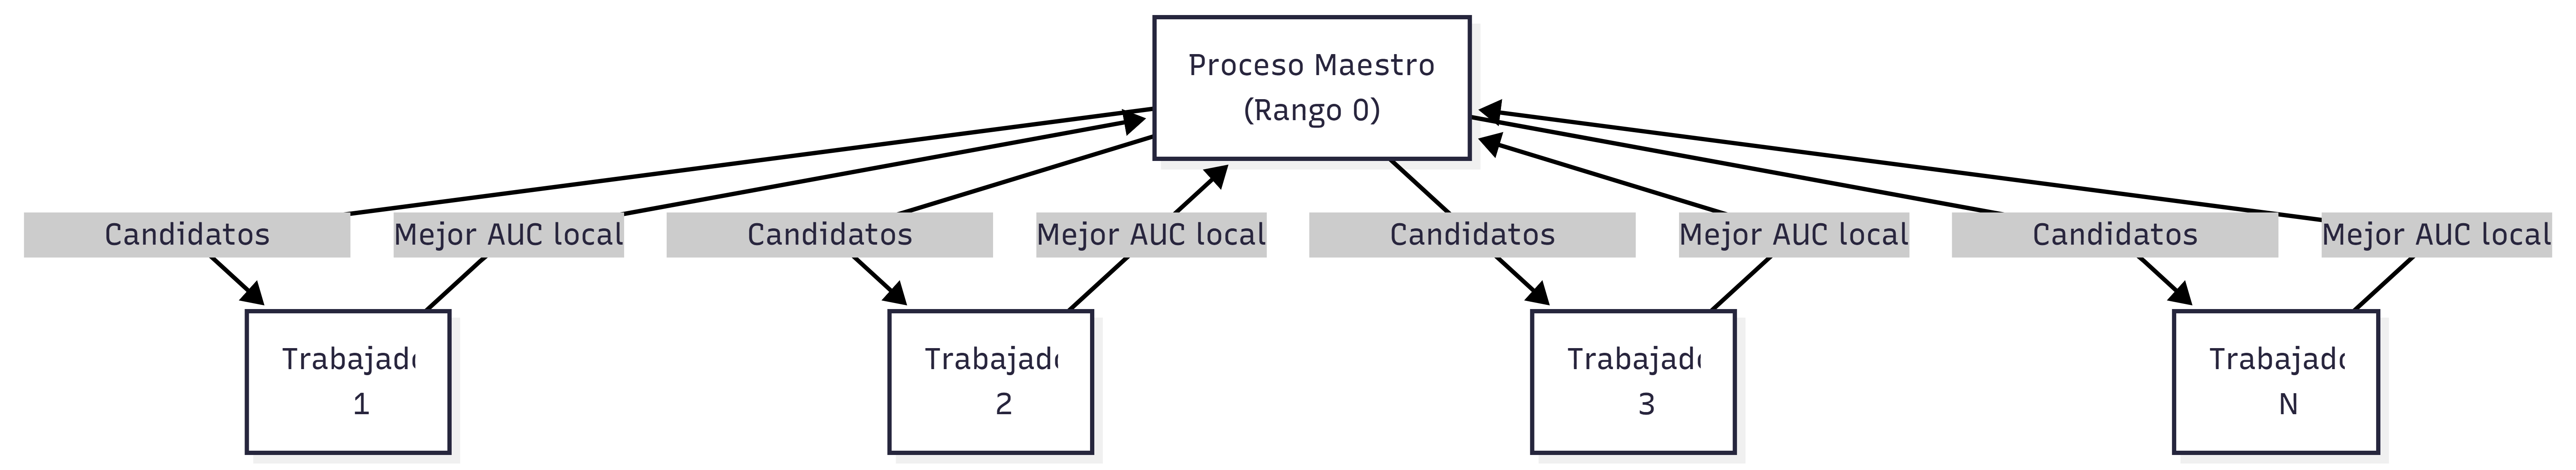
\includegraphics[width=0.85\textwidth]{figuras/implementaciones/01_mpi.png}
\caption{Arquitectura maestro--trabajadores mediante MPI.}
\label{fig:mpi_master_worker}
\end{figure}

\section{Flujo de Ejecución}

\begin{enumerate}
    \item Inicializar MPI.
    \item Obtener identificador del proceso.
    \item Distribuir candidatos.
    \item Evaluar subconjuntos.
    \item Comunicar resultados.
    \item Seleccionar el mejor AUC global.
    \item Finalizar MPI.
\end{enumerate}

\section{Pseudocódigo}

\begin{lstlisting}[language=C,
caption={Pseudocódigo general de la implementación MPI},
label={lst:mpi_pseudocode}]
MPI_Init();

if(rank == MASTER)
{
    distribuir_trabajo();
    recibir_resultados();
}
else
{
    recibir_datos();
    evaluar_candidatos();
    enviar_resultados();
}

MPI_Finalize();
\end{lstlisting}

\section{Ventajas}

\begin{itemize}
    \item Alta escalabilidad.
    \item Ejecución en múltiples nodos.
    \item Independencia de memoria.
\end{itemize}

\section{Limitaciones}

\begin{itemize}
    \item Overhead de comunicación.
    \item Mayor complejidad de implementación.
    \item Dependencia de infraestructura distribuida.
\end{itemize}

\section{Evidencias}

\begin{figure}[H]
\centering
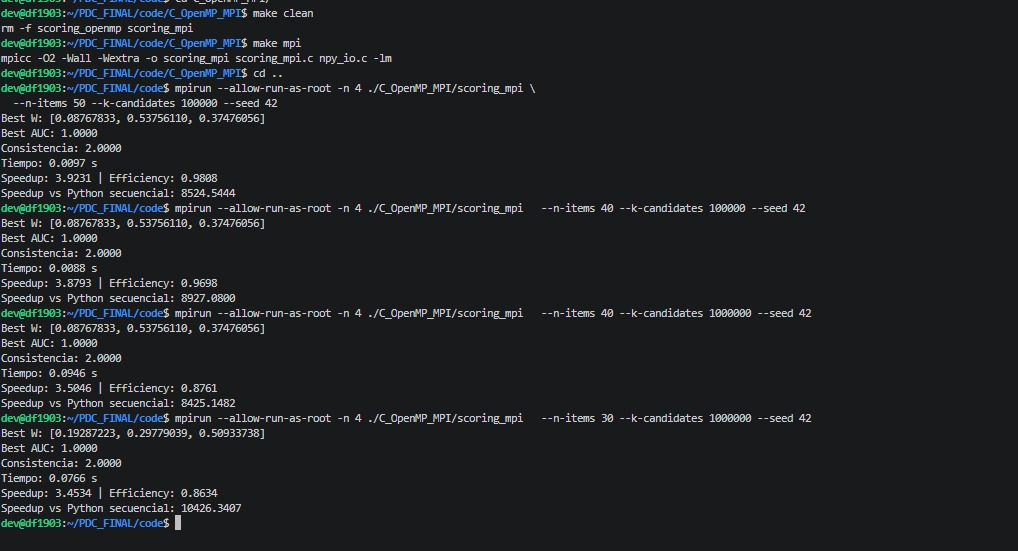
\includegraphics[width=0.90\textwidth]{figuras/capturas/mpi.png}
\caption{Resultados experimentales obtenidos mediante la implementación MPI.}
\label{fig:mpi_execution}
\end{figure}

\section{Compilación}

\begin{lstlisting}[language=bash,
caption={Compilación de la implementación MPI},
label={lst:mpi_compile}]
mpicc scoring_mpi.c -o scoring_mpi
\end{lstlisting}

\section{Ejecución}

\begin{lstlisting}[language=bash,
caption={Ejecución utilizando cuatro procesos MPI},
label={lst:mpi_run}]
mpirun -np 4 ./scoring_mpi
\end{lstlisting}